%! TEX program = xelatex
\documentclass[a4paper]{article}
\usepackage{amsmath, amssymb, mathtools}
\usepackage{amsthm}
\usepackage{fontspec}
\usepackage{xunicode}
\usepackage{fancyhdr}
\usepackage[french]{babel}
\usepackage[a4paper,centering]{geometry}
\usepackage{algorithm, algorithmic}
\usepackage{listings}
\usepackage{color}
\usepackage{graphicx}
\usepackage{enumitem}
\usepackage[export]{adjustbox}
\usepackage{multicol}
\usepackage{lastpage}
\usepackage[dvipsnames]{xcolor} 

\fancyhead[L, C, R]{}
\fancyfoot[L, R]{}
\fancyfoot[C]{\vspace{1mm}\thepage}
\lfoot{\vspace{1mm}Projet-LU2IN013}
\rfoot{\vspace{1mm}Sorbonne-université}
\rhead{\vspace{1mm}\today}
\lhead{\vspace{1mm}2022-2023}
\renewcommand{\headrulewidth}{1pt}
\renewcommand{\footrulewidth}{1pt}
\pagestyle{fancy}

\definecolor{gray}{rgb}{0.94, 0.94, 0.94}
\definecolor{red}{rgb}{0.6, 0, 0}
\xdefinecolor{mygreen}{RGB}{14,101,75}
\xdefinecolor{myred}{RGB}{140,23,19} 
\xdefinecolor{myblue}{RGB}{10,47,133} 

\lstset{
    numbers=left,
    numberstyle=\tiny, 
    backgroundcolor=\color{gray},
    language=Python,
    keywordstyle=\color{red},
    breaklines=true,
    frame=leftline,
    tabsize=4,
}

\begin{document}

\thispagestyle{plain}

\begin{titlepage}
    \begin{center}

        \bigskip
        
\includegraphics[scale=0.5]{logo_su.jpg}~\\[4cm]

        {\LARGE Rapport du projet LU2IN013}\\[0.3cm]
        \rule{\linewidth}{0.5mm} \\[0.6cm]
        {\huge \textbf{Composition modulaire des polynômes à une variable}}\\[0.4cm]
        \rule{\linewidth}{0.5mm} \\[1cm]
        {\large Encadrant : M. Vincent NEIGER}\\[5cm]

        {\Large Serigne Fallou FALL, Marie BONBOIRE}
        
        \vfill
        Février 2023 - Juin 2023


    \end{center}
\end{titlepage}

\newpage

\tableofcontents

\newpage


\section{INTRODUCTION}

\subsection{Sujet}
\textit{
Les polynômes à une variable sont un objet mathématique fondamental, qui
apparaît de manière omniprésente dans de nombreux problèmes et applications provenant
de contextes scientifiques variés. Par conséquent, les opérations les plus courantes sur les
polynômes sur les polynômes (addition, multiplication, division euclidienne, PGCD, inversion
modulaire, factorisation...) forment une composante essentielle de solutions algorithmiques et
logicielles conçues pour répondre aux besoins de ces contextes.
Les sciences du numérique fournissent un champ naturel d’applications pour ce type de calculs,
avec en particulier la cryptologie et les codes correcteurs d’erreurs où les calculs se font sur des
nombres exacts (entiers, rationnels, corps finis, ..). Par ailleurs, ces domaines demandent souvent
de résoudre des instances dont la taille est particulièrement importante. Il est donc essentiel de
disposer d’implantations haute-performance pour ce type de calculs. Ces implantations doivent
sélectionner l’algorithme le plus approprié, et exploiter au mieux les techniques disponibles sur
les processeurs modernes.
Dans le cadre de ce projet, on s’intéressera à l’opération de composition modulaire, qui occupe
une place importante notamment dans la factorisation des polynômes à une variable. On
étudiera puis implantera plusieurs algorithmes, allant du naïf, à celui qui est classiquement
implanté, puis enfin à celui qui a la meilleur complexité connue à ce jour. On mettra en
lumière la corrélation entre complexité estimée et performances en pratique, dans plusieurs cas
particuliers importants pour les applications à la factorisation. Enfin, si le temps le permet, on
exploitera des techniques de parallélisation ou de vectorisation pour améliorer les performances
pratiques.
Les étudiants développeront des compétences en algorithmique mathématique et en program-
mation haute-performance en langage C/C++. Ils seront initiés à l’usage d’outils collaboratifs
comme Git et à l’écriture scientifique avec LaTeX.
} REECRIRE

\subsubsection*{Objectifs du projet}

L'étude de notre projet se base spécialement sur les calculs arithmétiques des polynômes à une variable et notamment sur la composition modulaire. Nos objectifs principaux sont :
\begin{itemize}
	\item comprendre ce qu'est la composition modulaire de polynômes dans le corps ${\mathbb{Z}/p \mathbb{Z}}$
	\item trouver les algorithmes nous permettant de faire les calculs 
	\item connaitre les complexités et l'efficacité de ces algorithmes
	\item savoir comment les implémenter en langage informatique 
	\item en déduire l'utilité d'utiliser ces algorithmes et les perspectives qu'ils peuvent apporter en pratique

\end{itemize}

\subsection{Choix d'implantation}

\begin{itemize}
    \item SageMath : Logiciel open source mathématique.
    \item FLINT (Fast LIbrary for Number Theory) : Bibliothèque C fournissant des opérations arithmétiques sur les anneaux standards.
    \item NTL (Number Theory Library) : Bibliothèque C++ fournissant structures de données et algorithmes sur les entiers et les corps finis.
\end{itemize}

Nous avons commencé par implémenter les premières opérations arithmétiques (addition, soustraction, division euclidienne) en C à l'aide de la bibliothèque FLINT afin de mettre en pratique nos connaissances déjà acquises dans ce langage.
Toutefois, il s'est avéré beaucoup plus pratique de coder en Python sur SageMath puisque nous n'avons pas à nous occuper de la gestion de la mémoire.
Nous nous sommes donc centrés sur cette implantation durant la suite du projet.

Notamment grace à des fonctions de précalcul, la composition modulaire est plus perfomante en C++ avec l'utilisation de la bibliothèque NTL.
Certains algorithmes nous étaient fournis dans la bibliothèque NTL. Il a donc été intéressant de comparer notre implémentation SageMath avec ces derniers.


\subsection{Premières notions et notations}

\subsubsection*{Arithmétique modulaire sur les polynômes}

L'arithmétique s'agit essentiellement de l'étude des nombres et des opérations élémentaires comme l'addition, la soustraction, la multiplication, et la division. 
Ainsi, plusieurs outils sont utilisés comme la division euclidienne, le calcul du PGCD, l'inversion modulaire avec l'algorithme d'Euclide, le théorème de Bézout. C'est à partir de l'arithmétique que nous avons recueilli plusieurs notions dans notre étude que nous allons détailler.

\paragraph{Corps d'étude :} ${\mathbb{Z}/p \mathbb{Z}}[x] := \{\text{polynômes univariés à coefficients entiers dans }\{0,...,p-1\}\}$ où $p$ est un nombre premier tenant dans un mot machine (i.e. 64 bits ?). \\
Nous avons fait ce choix pour obtenir un contexte exacte de ce qui se passe. Cela s'oppose à un contexte numérique que nous rencontrons avec les corps $\mathbb{Q}$ et $\mathbb{R}$ par exemples.	

\textit{
\paragraph{Algorithme d'Euclide, calcul de PGCD et division euclidienne} :
Si A et B sont deux polynômes, il existe un polynôme Q et un polynôme R tels que  
\[
A(x) = Q(x)\cdot B(x) + R(x) \text{ avec } deg(R(x)) < deg(B(x))
\]
La division euclidienne est utilisée dans divers domaines mathématique et informatique tels que le calcul du PGCD, la recherche de nombres premiers et et de calcul modulo. Ainsi, son utilité principal dans ${\mathbb{Z}/p \mathbb{Z}}$ est la simplification des expressions et la détermination de propriétés spécifiques des polynômes. Elle est utile pour simplifier les expressions, factoriser les polynômes, trouver des racines, résoudre des équations polynomiales, établir des critères de divisibilité et également effectuer des opérations sur les polynômes et analyser leurs propriétés.
} 
A REVOIR

\subsubsection*{Notations}
\begin{itemize}
\item $\tilde{O}$ : cache les facteurs logarithmiques dans la complexité des algorithmes (\textit{ie} $\tilde{O}(c)$ = $O(c\cdot log^{k}(c))$ pour $k>0$)
\item $\omega$ : c'est le plus petit nombre réel tels que deux matrices carrées de taille $n$ peuvent être multipliées. Pour notre étude, nous avons choisi la valeur donnée par V.Strassen soit $\omega=2.807$
La multiplication de deux matrices carrées de taille $n$ se fait donc en $O(n^\omega)=O(n^{2.807})$
\end{itemize}


\section{MULTIPLICATION}

La multiplication est une opération de base qui intervient beaucoup dans la manipulation de polynômes.

Dans cette section, nous étudions deux algorithmes qui calculent le produit de deux polynômes univariés $f,g \in \mathbb{Z}/p\mathbb{Z}[x]$ de degré strictement inférieur à $n$ :
\[
f(x)=f_0+f_1x+...+f_{n-1}x^{n-1}\text{ et }g(x)=g_0+g_1x+...+g_{n-1}x^{n-1}
\]

\subsection{Algorithme naif}

Ce premier algorithme consiste à simplement développer le produit des coefficients :
\[
(f\cdot g)(x)=(f_0+f_1x+...+f_{n-1}x^{n-1})\cdot (g_0+g_1x+...+g_{n-1}x^{n-1})=\sum_{i=0}^{2n-2} (\sum_{j+k=i}f_j\cdot g_k) x^i
\]

\begin{lstlisting}[title={multiplication naive}]
    def mult_naive(f, g) :
    ring = f.parent()

    #initialisation de la liste des coefficients
    res = [0]*(f.degree()+g.degree()+1) 
    
    for i in range(0, f.degree()+1):
        for j in range(0, g.degree()+1):
            res[i+j] += f[i]*g[j]

    return ring(res) 
\end{lstlisting}

\subsubsection*{Complexité}
\begin{itemize} 
    \item $f$ et $g$ sont de degré au plus $n$, ils ont donc chacun au plus $n$ coefficients
\end{itemize}
L'algorithme naïf est en $$(n-1)\cdot (n-1) = n^2 - 2n + 1 \Longrightarrow O(n^2)$$

\subsection{Algorithme de Karatsuba}

L'amélioration proposée par Karatsuba repose sur le fait de scinder les polynomes selon :
\[
f(x)=f^{(0)}+f^{(1)}x^k\text{ et }g(x) = g^{(0)}+g^{(1)}x^k
\]
avec $f^{(0)}, f^{(1)}, g^{(0)}, g^{(1)}$ de degré au plus $k-1$ et $k=\lceil n/2 \rceil$. \\

Le produit s'écrit alors :
\[
(f\cdot g)(x) = \textcolor{myred}{(f^{(0)}\cdot g^{(0)})}
+\left(\textcolor{mygreen}{(f^{(0)}+f^{(1)})\cdot (g^{(0)} + g^{(1)})} - f^{(0)}\cdot g^{(0)} - f^{(1)}\cdot g^{(1)}\right)x^k+
\textcolor{myblue}{(f^{(1)}\cdot g^{(1)})}x^{2k} 
\]

Notons qu'en développant le produit \textcolor{mygreen}{vert}, nous retombons sur l'algorithme naïf 
\begin{align*}
(f\cdot g)(x) &= (f^{(0)}\cdot g^{(0)})
        +(f^{(0)}\cdot g^{(1)}+f^{(1)}\cdot g^{(0)})x^k+
        (f^{(1)}\cdot g^{(1)})x^{2k} \\
        &= (f^{(0)}+f^{(1)}x^k) \cdot (g^{(0)}+g^{(1)})x^k
\end{align*}

Ainsi, l'algorithme de Karatsuba permet de gagner une multiplication. Par le biais des appels récursifs, ce gain va apparaître dans la complexité.

\begin{lstlisting}[title={Karatsuba}]
def karatsuba(f, g) :
    ring = f.parent()

    #cas de base
    if f.is_zero() : return f
    if g.is_zero() : return g
    
    #seuil 
    if (f.degree() <= 10 and g.degree() <= 10) : 
        return mult_naive(f, g)

    k = max(f.degree()/2, g.degree()/2).ceil()

    #extraction des sous polynômes
    f0 = ring(f.list()[:k]); f1 = ring(f.list()[k:])
    g0 = ring(g.list()[:k]); g1 = ring(g.list()[k:])

    #opérations de l'algorithme
    h1 = karatsuba(f0, g0)
    h2 = karatsuba(f1, g1)
    h5 = karatsuba(f0+f1, g0+g1)
    h7 = h5 - h1 - h2

    h = h1 + h7.shift(k) + h2.shift(2*k)

    return h
\end{lstlisting}

\subsubsection*{Complexité}
\begin{itemize}
    \item Calcul récursif 3 multiplications de polynômes de degré au plus $k-1$
    \item Soit $C_n$ le nombre de tests effectués avant l'appel de la fonction multiplication naive:
    $$C_n = 3\times{C_{\lceil n/2 \rceil}} + 1 = 3\times{C_{2^{k-1}}} + 1 \text{ avec } k = log_2(n) \text{ ... }$$
    $$\Longrightarrow C_n = \dfrac{3^{k+1} - 1}{2} = \dfrac{3\times{3}^{log_2(n)} - 1}{2} = \dfrac{3\times{n}^{log_2(3)} - 1}{2} $$
    
\end{itemize}
L'algorithme de Karatsuba est en $O(n^{log_2(3)}) \approx O(n^{1,59})$

\subsection{Comparaisons}

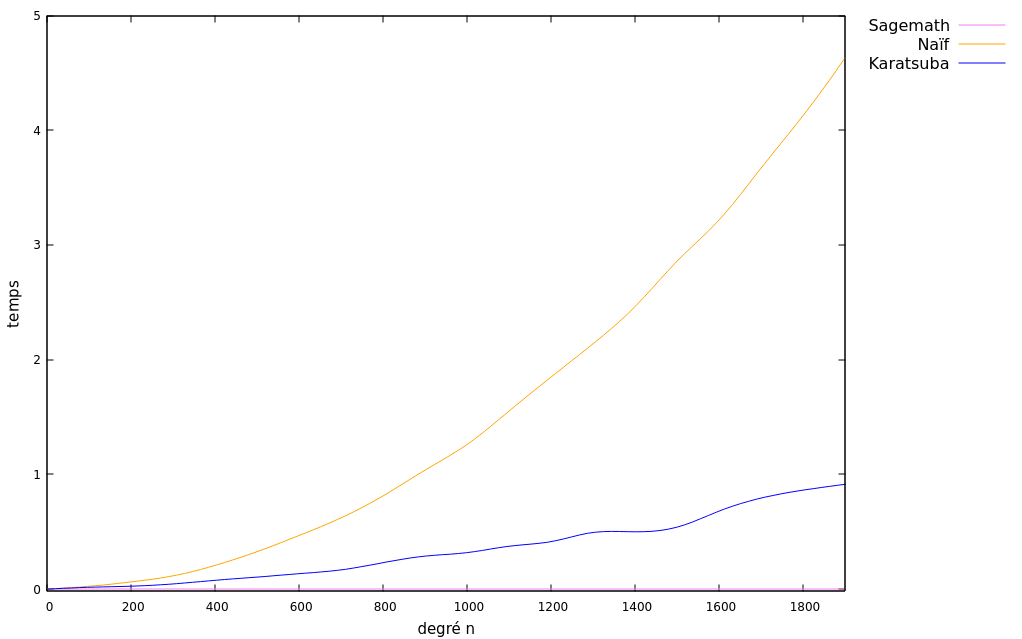
\includegraphics[scale=0.5, center]{multi.png}
\textit{
\begin{itemize}
    \item Le graphe ci-dessus nous montre l'allure cubique de la courbe de l'algorithme naif qui a une complexité moins optimale que celui de Karatsuba qui présente une allure quadratique. Cependant, la version déjà implémenté sur sagemath reste nettement le plus optimisé.
\end{itemize}
}

Le produit effectué par SageMath utilise un algorithme à base de FFT.


\theoremstyle{definition}
\newtheorem*{thm}{Theoreme}
\begin{thm}
La multiplication de polynômes de degré au plus $n$ dans $\mathbb{Z}/p\mathbb{Z}$ requiert $O(nlognloglogn)$ opérations via la transformée de Fourier rapide (FFT).
\cite{aecf-2017-livre}
\end{thm}

Cette première section nous a donc montré l'importance du choix de l'algorithme dans les opérations sur les polynômes.


\section{ALGORITHMES DE COMPOSITION MODULAIRE}

L'enjeu de la composition modulaire est que nous n'arrivons pas à obtenir une complexité quasi linéaire.
Dans cette autre section du rapport, nous nous intéressons donc à l'étude et la comparaison de trois algorithmes de composition modulaire qui calculent g(a) mod f avec 
$f \in \mathbb{Z}/p\mathbb{Z}[x]$ de degré $n$, $a \in \mathbb{Z}/p\mathbb{Z}[x]$ de degré au plus $n$ et $g \in \mathbb{Z}/p\mathbb{Z}[y]$ de degré au plus $n$.



\subsection{Algorithme naïf}

L'algorithme naïf de composition modulaire consiste à directement évaluer g en a et à retourner le résultat en le réduisant par f :
\[
g(a)\text{ mod }f = \left(\sum_{k=0}^n g_k \cdot a^k\right) \text{ mod }f    
\]

\begin{lstlisting}[title={naive}]
def eval_naive(g, a, f) :
	ring = g.parent()

	res = ring(g[0])
	ai = a
	
    for i in range(1, g.degree()+1) :
		res = res + g[i]*ai
		ai = a*ai

	return res % f
\end{lstlisting}

\subsubsection*{Complexité}
\begin{itemize}
    \item Pour $i \in \{0,...,n\}$, le degré des $a_i$ est au plus égal à $i(n-1)$ donc, le produit $a_i=a_{i-1}\cdot a$ est en $\tilde{O}(in)$ (ref th)
    \item Nous effectuons $n$ tours de boucles donc $n$ multiplications
\end{itemize}
La complexité de l'algotihme naïf est :
\[
\sum_{i=1}^{n}in=n \cdot \dfrac{n(n+1)}{2} \Longrightarrow \tilde{O}(n^3)
\]

\subsection{Algorithme d'Horner}

\[
g(a)\text{ mod }f = ((...((((g_{n-1}\cdot a)\text{ mod }f\ +\ g_{n-2})\cdot a)\text{ mod }f\ +\ g_{n-3})...)\cdot a)\text{ mod }f\ +\ g_0
\]

\begin{lstlisting}[title={Horner}]
    def horner(g, a, f) :
        res = g[g.degree()]
        for i in range(g.degree()-1, -1, -1) :
            res = (res*a)%f + g[i]
        return res%f
\end{lstlisting}

\subsubsection*{Complexité}
\begin{itemize}
    \item Pour $i \in \{0,...,n\}$, le degré de $a_i$ mod $f$ est au plus égal à $n$ donc, le produit $a_i=a_{i-1}\cdot a$ est en $\tilde{O}(n)$ (ref th)
    \item Nous effectuons $n$ tours de boucles donc $n$ multiplications
\end{itemize}
La complexité de l'algorithme d'Horner est :
\[
\sum_{i=1}^n n=n\cdot \sum_{i=1}^n 1 = n\cdot n\Longrightarrow \tilde{O}(n^2)
\]

\subsection{Algorithme de Brent et Kung}

L'avancée de Brent et Kung a été de considérer le produit bien connu de deux matrices à coefficients constants $\omega$.


Soit $\delta = \sqrt{n}$. Nous écrivons $g$ sous la forme de :
\begin{align*}
    g(y) &= g_0 + g_1y + ... + g_{\delta-1}y^{\delta-1} \\
        &+ y^\delta(g_\delta + g_{\delta+1}y + ... + g_{2\delta-1}y^{\delta-1}) \\
                                      &+ y^{2\delta}(g_{2\delta} + g_{2\delta+1}y + ... + g_{3\delta-1}y^{\delta-1}) \\
                                      &+ ... \\
                                      &+ y^{\delta(\delta-1)}(g_{\delta(\delta-1)} + g_{\delta(\delta-1)+1}y + ... + g_{\delta^2-1}y^{\delta-1}) 
\end{align*}

Nous transformons alors cette expression en produit de matrices dont une est à coefficients constants :
\[
g(y) = 
\begin{pmatrix}
    1 & y^\delta & ... & (y^\delta)^{\delta-1}  \\  
\end{pmatrix}
\begin{pmatrix}
    g_0 & g_1 & ... & g_{\delta-1} \\
    g_{\delta} & g_{\delta+1} & ... & g_{2\delta-1} \\
    \vdots & ... & \vdots \\
    g_{\delta(\delta-1)} & g_{\delta(\delta-1)+1} & ... & g_{\delta^2-1}
\end{pmatrix}
\begin{pmatrix}
    1 \\
    y \\
    \vdots \\
    y^{\delta-1}
\end{pmatrix}
\]

De même, nous transformons le vecteur des $\delta$ puissances de $a$ mod $f$, en un produit d'une matrice à coefficients constants par un vecteur de l'inconnue $x$ :
\[
    \begin{pmatrix}
        1 \\
        a \text{ mod }f\\
        \vdots \\
        a^{\delta-1} \text{ mod }f
    \end{pmatrix}
    =
    \begin{pmatrix}
        1 & 0 & ... & 0 \\
        a_{1,0} & a_{1,1} & ... & a_{1,n-1} \\
        \vdots & \vdots & ... & \vdots \\
        a_{\delta-1,0} & a_{\delta-1,1} & ... & a_{\delta-1,n-1}
    \end{pmatrix}
    \begin{pmatrix}
        1 \\
        x \\
        \vdots \\
        x^{n-1}
    \end{pmatrix}
\]

Nous obtenons ainsi la formule suivante :
\[
g(a)\text{ mod }f =
\begin{pmatrix}
    1 & y^\delta & ... & (y^\delta)^{\delta-1}  \\  
\end{pmatrix}
\begin{pmatrix}
    g_0 & ... & g_{\delta-1} \\
    g_{\delta} & ... & g_{2\delta-1} \\
    \vdots & ... & \vdots \\
    g_{\delta(\delta-1)} & ... & g_{\delta^2-1}
\end{pmatrix}
\begin{pmatrix}
    1 &  ... & 0 \\
    a_{1,0} & ... & a_{1,n-1} \\
    \vdots &  ... & \vdots \\
    a_{\delta-1,0} & ... & a_{\delta-1,n-1}
\end{pmatrix}
\begin{pmatrix}
    1 \\
    x \\
    \vdots \\
    x^{n-1}
\end{pmatrix}
\]


\begin{lstlisting}[title={brent and kung}]
def brentkung(g, a, f) :

	ring = a.parent()
	d = g.degree()+1; n = f.degree()
	if a.degree() >= n:
		raise ValueError("Erreur: a de degré trop élevé")

    #choix de r et s tels que r*s >= n
	r = RR(d.sqrt()).ceil()
	s = RR(d/r).ceil()

    #calcul des puissances de a
	ac = [ring(0)]*(r+1)
	ac[0] = ring(1)
	for i in range(1, r+1) :
		ac[i] = (a*ac[i-1]) % f

    #calcul du produit matriciel
	ma = matrix(r, n, [(ac[i])[j] for i in range(r) for j in range(n)])
	mg = matrix(s, r, [g[i*r+j] for i in range(s) for j in range(r)])
	mb = mg*ma

    #liste coefficients -> polynôme
	b = [ring(0)]*s
	for i in range(s) :
		b[i] = ring(mb[i].list())

	res = b[0]
	ar = ac[r]

	res = horner(b, ar, f)
	return res
\end{lstlisting}

Dans notre rapport, nous avons choisi $ r = s = \delta = \sqrt{n}$ afin de simplifier la notation de la complexité.

\subsubsection*{Complexité}
\begin{itemize}
    \item Pour $i \in \{0,...,\delta\}$, le degré de $a_i$ mod $f$ est au plus égal à $n$ donc, le produit $a_i=a_{i-1}\cdot a$ est en $\tilde{O}(n)$ (ref th)
    \item La matrice des coefficients constants de $a$ est implicitement découpée en $\sqrt{n}$ matrices carrées de dimension $\sqrt{n}$.
    Nous avons donc $\sqrt{n}$ produits de matrices en $$O(\sqrt{n}\cdot \sqrt{n}^{\omega})=O(n^{(\omega+1)/2})$$ 
    \item L'évaluation polynômiale d'Horner coûte $O(n\cdot \delta)=O(n^{3/2})$
\end{itemize}
La complexité de l'algorithme de Brent et Kung est donc donnée par :
\[
n < n^{3/2} < n^{(\omega+1)/2}= n^{1,9035} \Longrightarrow O(n^{1,9035})
\]

\newpage

\subsection{Comparaisons}
\begin{multicols}{2}
    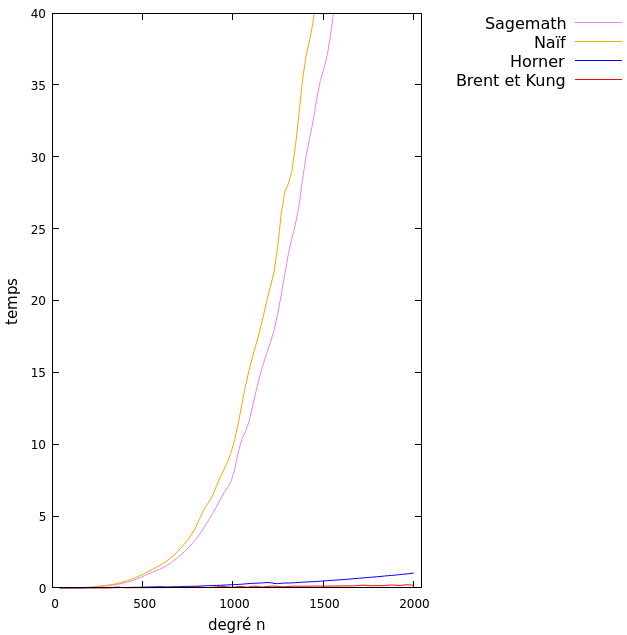
\includegraphics[scale=0.4, center]{comp.png}
    \columnbreak

    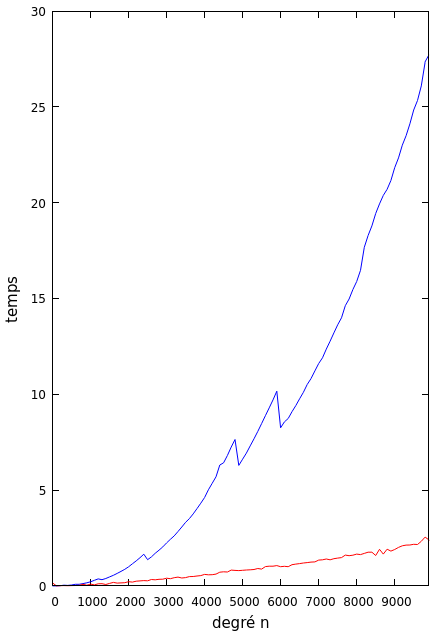
\includegraphics[scale=0.4, center]{comp_2.png}
\end{multicols}
\textit{
\begin{itemize}
    \item Le premier graphe nous montre une vision plus large sur la différence entre les différents algorithmes. Bien vrai que l'algorithme de sagemath soit légèrement plus meilleur en complexité temporelle que celui du naif, on remarque une nette différence entre ces deux algorithmes qui sont de complexité cubique par rapport à ceux de Horner et Brent et Kung qui se rapprochent plus de l'ordre quadratique en complexité.
    \item Le deuxième graphe nous permet de déduire pour des polynomes de degré assez grand que Brent et Kung reste l'algorithme avec la meilleur complexité pour la composition modulaire. Les pics dans le graphe relèvent de l'implémentation des algorithmes en sagemath qui peut générer des calculs implicites.
\end{itemize}
}

\section{ALGORITHME DE NUSKEN ET ZIEGLER}

L'algorithme de Nüsken et Ziegler est une généralisation de celui de Brent et Kung aux polynômes à deux variables. 
Son principe est donc similaire, en différant au niveau de la matrice des coefficients de $g$ qui ici, contient des polynomes en $x$.
Nous y retrouvons toutefois les mêmes étapes de calcul.

\[
g(x,y) = \sum_{i,j<\delta}g_{i+\delta j}(x)y^{i+\delta j} = \sum_{j<\delta} \left( \sum_{i<\delta} g_{i+\delta j}(x)y^i \right) y^{\delta j}     
\]
\[
g(x, a)\text{ mod }f =
\begin{pmatrix}
    1 & y^\delta & ... & (y^\delta)^{\delta-1}  \\  
\end{pmatrix}
\begin{pmatrix}
    g_0(x) & ... & g_{\delta-1}(x) \\
    g_{\delta}(x) & ... & g_{2\delta-1}(x) \\
    \vdots & ... & \vdots \\
    g_{\delta(\delta-1)}(x) & ... & g_{\delta^2-1}(x)
\end{pmatrix}
\begin{pmatrix}
    1 &  ... & 0 \\
    a_{1,0} & ... & a_{1,n-1} \\
    \vdots &  ... & \vdots \\
    a_{\delta-1,0} & ... & a_{\delta-1,n-1}
\end{pmatrix}
\begin{pmatrix}
    1 \\
    x \\
    \vdots \\
    x^{n-1}
\end{pmatrix}
\]

\bigskip

\begin{lstlisting}[title={nusken et ziegler}]
def nuskenziegler(g, a, f) :
    ring = a.parent()
    d = RR(sqrt(g.degree()+1)).ceil()

    #réécriture
    ringY = g.parent().univariate_ring(y)
    lg = ringY(g)

    #calcul du produit matriciel
    mg = matrix(d, d, [lg[i+d*j](X) for j in range(d) for i in range(d) ])

    ac = [ring(0)]*d
    ac[0] = ring(1)
    for i in range(1, d) :
        ac[i] = (a*ac[i-1]) % f

    ma = vector(ac)
    mr = mg*ma

    r = [ring(0)]*d
    for j in range(d) :
        r[j] = ring(mr[j].list()) %f
    
    res = horner(r, ac[d], f)

    return res
\end{lstlisting}

\subsubsection*{Complexité}
\begin{itemize}
    \item Pour $i \in \{0,...,\delta\}$, le degré de $a_i$ mod $f$ est au plus égal à $n$ donc, le produit $a_i=a_{i-1}\cdot a$ est en $\tilde{O}(n)$
    \item Soit $d$ le degré de la variable $x$, on a $\sqrt{n}$ de produits de matrice pour la variable $y$ et $d$ produits de matrice pour la variable $x$
    Nous avons donc $\sqrt{n} + d$ produits de matrices en $$O((\sqrt{n}+d)\cdot \sqrt{n}^{\omega})=O(n^{(\omega+1)/2} + n^{(\omega/2)}\cdot d)$$ 
    \item L'évaluation polynômiale d'Horner coûte $O(n\cdot \delta)=O(n^{3/2})$
\end{itemize}
La complexité de l'algorithme de Nusken et Ziegler est donné par:
\[
\Longrightarrow O(n + n^{3/2} + n^{(\omega+1)/2} + n^{(\omega/2)}\cdot d) \approx O(n^{(\omega/2)}\cdot (\sqrt{n}+d))
\]
Donc si le degré de $d<\sqrt{n}$, on se ramène à la même complexité que Brent et kung
\[
n^{(\omega+1)/2} + n^{(\omega/2)}\cdot d < 2\times{n}^{(\omega+1)/2} = 2\times{n}^{1,9035} \Longrightarrow O(n^{1,9035})
\]

\bigskip
\section{BIBLIOGRAPHIE}

\nocite{*}

\bibliographystyle{plain}
\bibliography{biblio}

\subsection*{Lien GitHub} 
https://github.com/marizee/Projet-LU2IN013-2023

\end{document}
